\documentclass{beamer}
\usepackage[utf8]{inputenc}
\usetheme{Singapore}
\usecolortheme{default}
\beamertemplatenavigationsymbolsempty
\usepackage{multimedia, hyperref}

\title[Dinamica molecolare] 
{Esercizio dinamica molecolare}

\author[Lorenzo Tasca]
{Lorenzo Tasca}

\institute[]
{
  Dipartimento di Fisica “Giuseppe Occhialini”\\
  Università degli Studi di Milano-Bicocca\\
}

\date[04/2024] 
{Aprile 2024 }



\begin{document}

\frame{\titlepage}

\begin{frame}
    \frametitle{Sharp cutoff approach}

    \begin{center}
        \begin{itemize}
            \item $r_c = 4.5 \,\AA$,
            \item $T_{term} = 3\times 10^{-12}\,s$,
            \item $T_{tot} = 10 \times 10^{-12}\,s$,
            \item $\Delta t= 8 \times 10^{-15}\,s$,
            \item sharp cutoff at $r_c$.
        \end{itemize}
    \end{center}

\end{frame}

\begin{frame}
    \frametitle{Sharp cutoff approach, initial temperature}

    $$T_{init}=15\,K \rightarrow \langle T \rangle = 10.82\,K $$

    \begin{figure}
        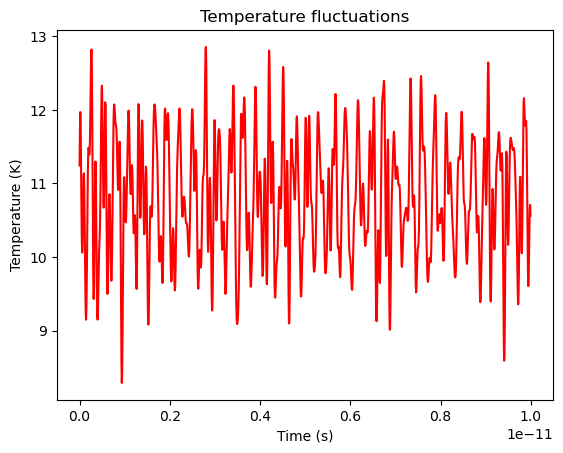
\includegraphics[width=0.7\textwidth]{images/temp1.png}
    \end{figure}

\end{frame}

\begin{frame}
    \frametitle{Sharp cutoff approach, initial temperature}

    $$T_{init}=15\,K \rightarrow \langle T \rangle = 10.82\,K $$

    \begin{figure}
        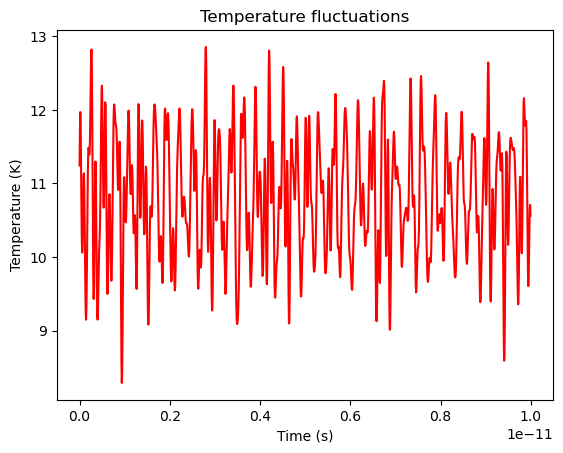
\includegraphics[width=0.7\textwidth]{images/tempafter.png}
    \end{figure}

\end{frame}


\begin{frame}
    \frametitle{Sharp cutoff approach, energy conservation}

    $$\frac{\delta E }{E}=6.5\times 10^{-7}    $$

    \begin{figure}
        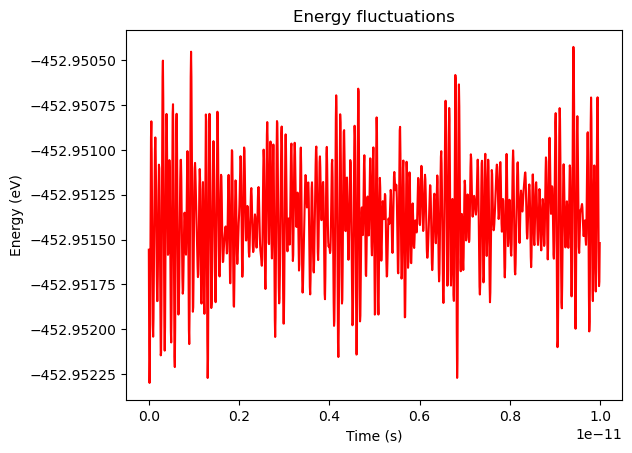
\includegraphics[width=0.7\textwidth]{images/energy1.png}
    \end{figure}

\end{frame}

\begin{frame}
    \frametitle{Sharp cutoff approach, velocity distribution}

    $$f(v_x)=\sqrt{\frac{M}{{2\pi k_B T}}} \exp {\left(-\frac{M\, v_x^2}{2 k_B T}\right)}$$

    \begin{figure}
        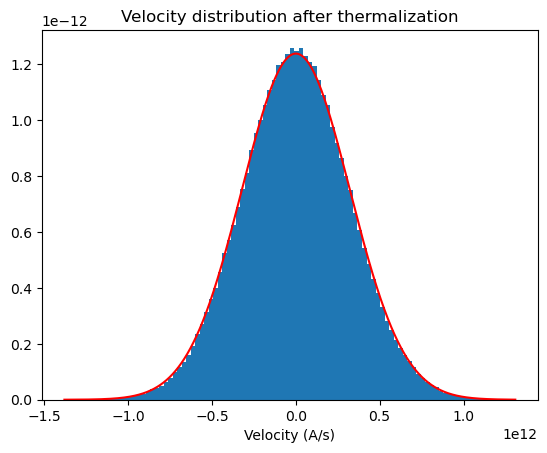
\includegraphics[width=0.7\textwidth]{images/distvelocity1.png}
    \end{figure}

\end{frame}


\begin{frame}
    \frametitle{Sharp cutoff approach, steepest descent}

    $$F_{max}<0.01\,eV/\AA$$

    \begin{figure}
        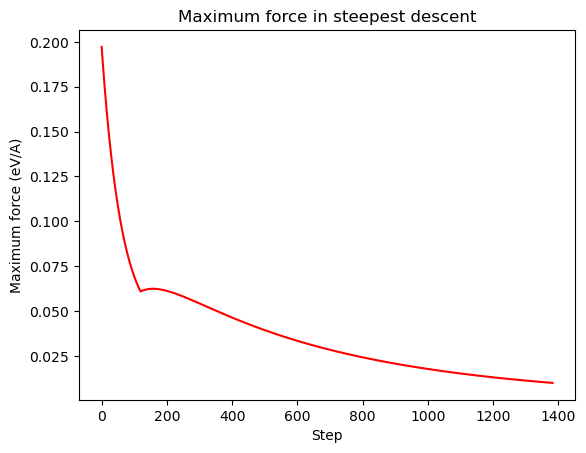
\includegraphics[width=0.7\textwidth]{images/force.png}
    \end{figure}

\end{frame}

\begin{frame}
    \frametitle{Sharp cutoff approach, steepest descent}

    $$F_{max}<0.01\,eV/\AA$$

    \begin{figure}
        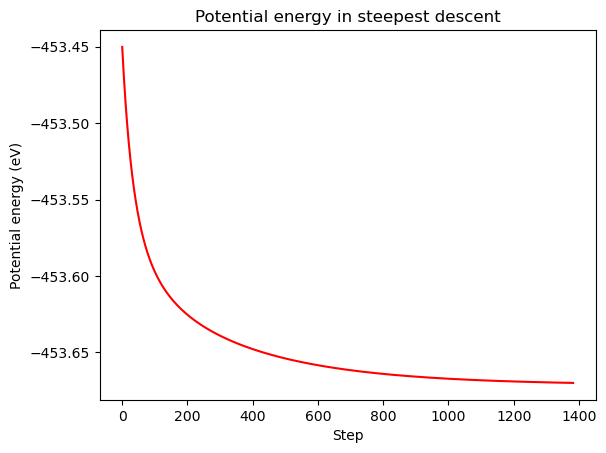
\includegraphics[width=0.7\textwidth]{images/Usteepest.png}
    \end{figure}

\end{frame}

\begin{frame}
    \frametitle{Sharp cutoff approach, steepest descent}

    $$T_{init}=20\,K \rightarrow \langle T \rangle = 10.06\,K $$

    \begin{figure}
        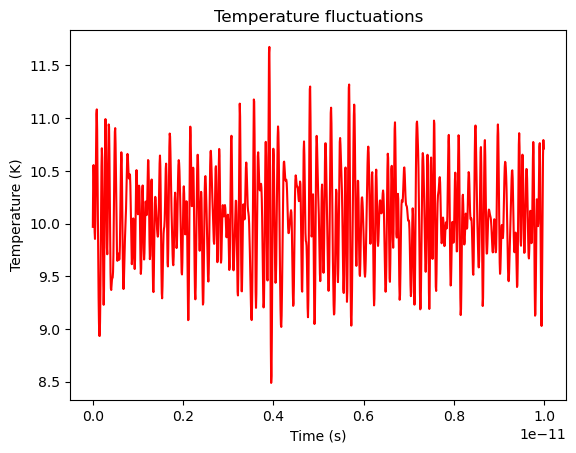
\includegraphics[width=0.7\textwidth]{images/tempforce.png}
    \end{figure}

\end{frame}


\begin{frame}
    \frametitle{Sharp cutoff approach, energy at higher temperatures}

    $$\langle T \rangle = 199.74\,K $$
    $$\frac{\delta E }{E}=1.54 \times 10^{-4}   $$

    \begin{figure}
        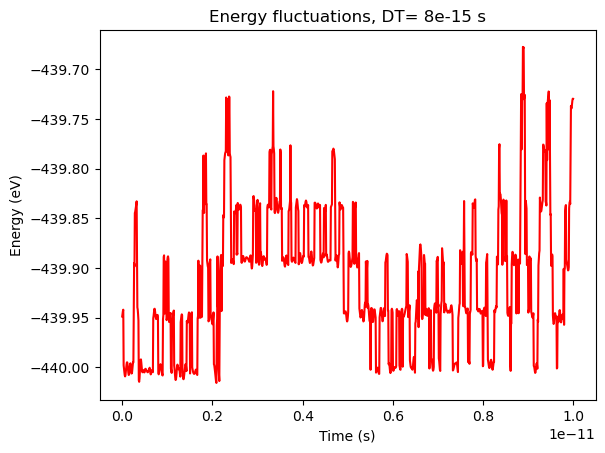
\includegraphics[width=0.7\textwidth]{images/awfulenergy.png}
    \end{figure}

\end{frame}

\begin{frame}
    \frametitle{Sharp cutoff approach, energy}

    \begin{center}
        Lowering the time step does not solve the problem
    \end{center}

    \begin{figure}
        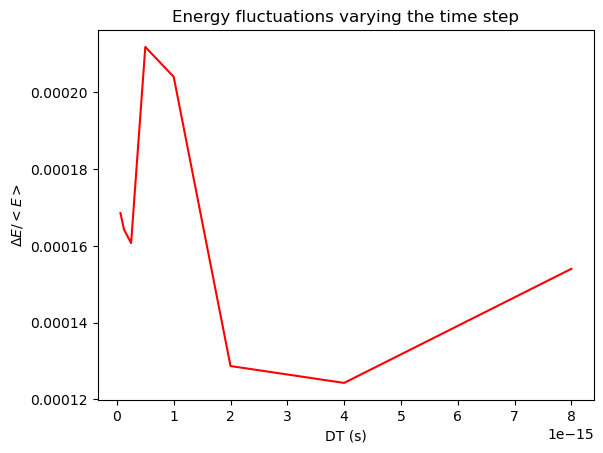
\includegraphics[width=0.7\textwidth]{images/lowertimestepawful.png}
    \end{figure}

\end{frame}

\begin{frame}
    \frametitle{Polynomial junction approach}

    Insert 7th order polynomial junction between $r'=4.2\,\AA$ and $r_c=4.5\,\AA$.
    \begin{figure}
        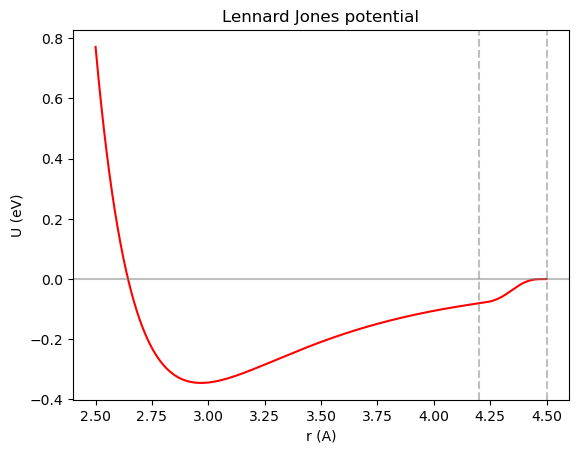
\includegraphics[width=0.7\textwidth]{images/LJ.png}
    \end{figure}

\end{frame}

\begin{frame}
    \frametitle{Polynomial junction approach, ideal timestep}

    Ideal timestep is $\Delta t = 8\times 10^{-15}\,s$ as it gives $\frac{\delta E}{E}= 1.08 \times 10^{-5}$.
    \begin{figure}
        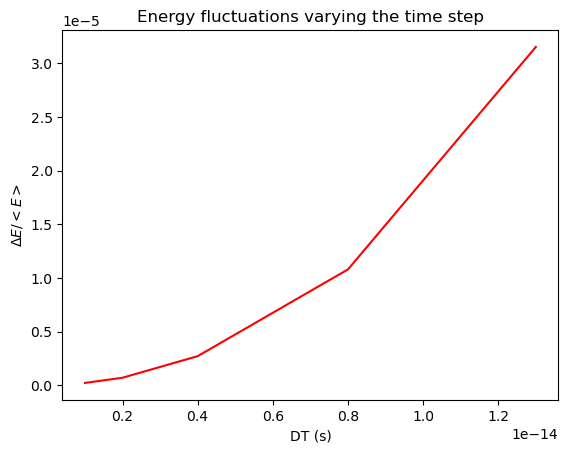
\includegraphics[width=0.7\textwidth]{images/lowertimestepamazing.png}
    \end{figure}

\end{frame}

\begin{frame}
    \frametitle{Polynomial junction approach, energy}

    $$\frac{\delta E}{E}= 1.08 \times 10^{-5}$$
    \begin{figure}
        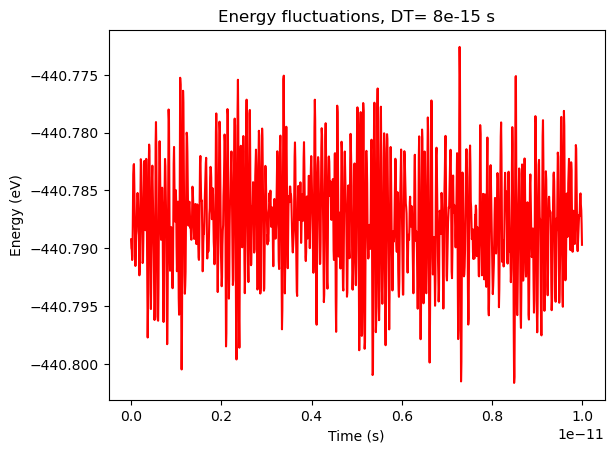
\includegraphics[width=0.7\textwidth]{images/energyjunction.png}
    \end{figure}

\end{frame}

\begin{frame}
    \frametitle{Polynomial junction approach, simulation}

    \begin{figure}
        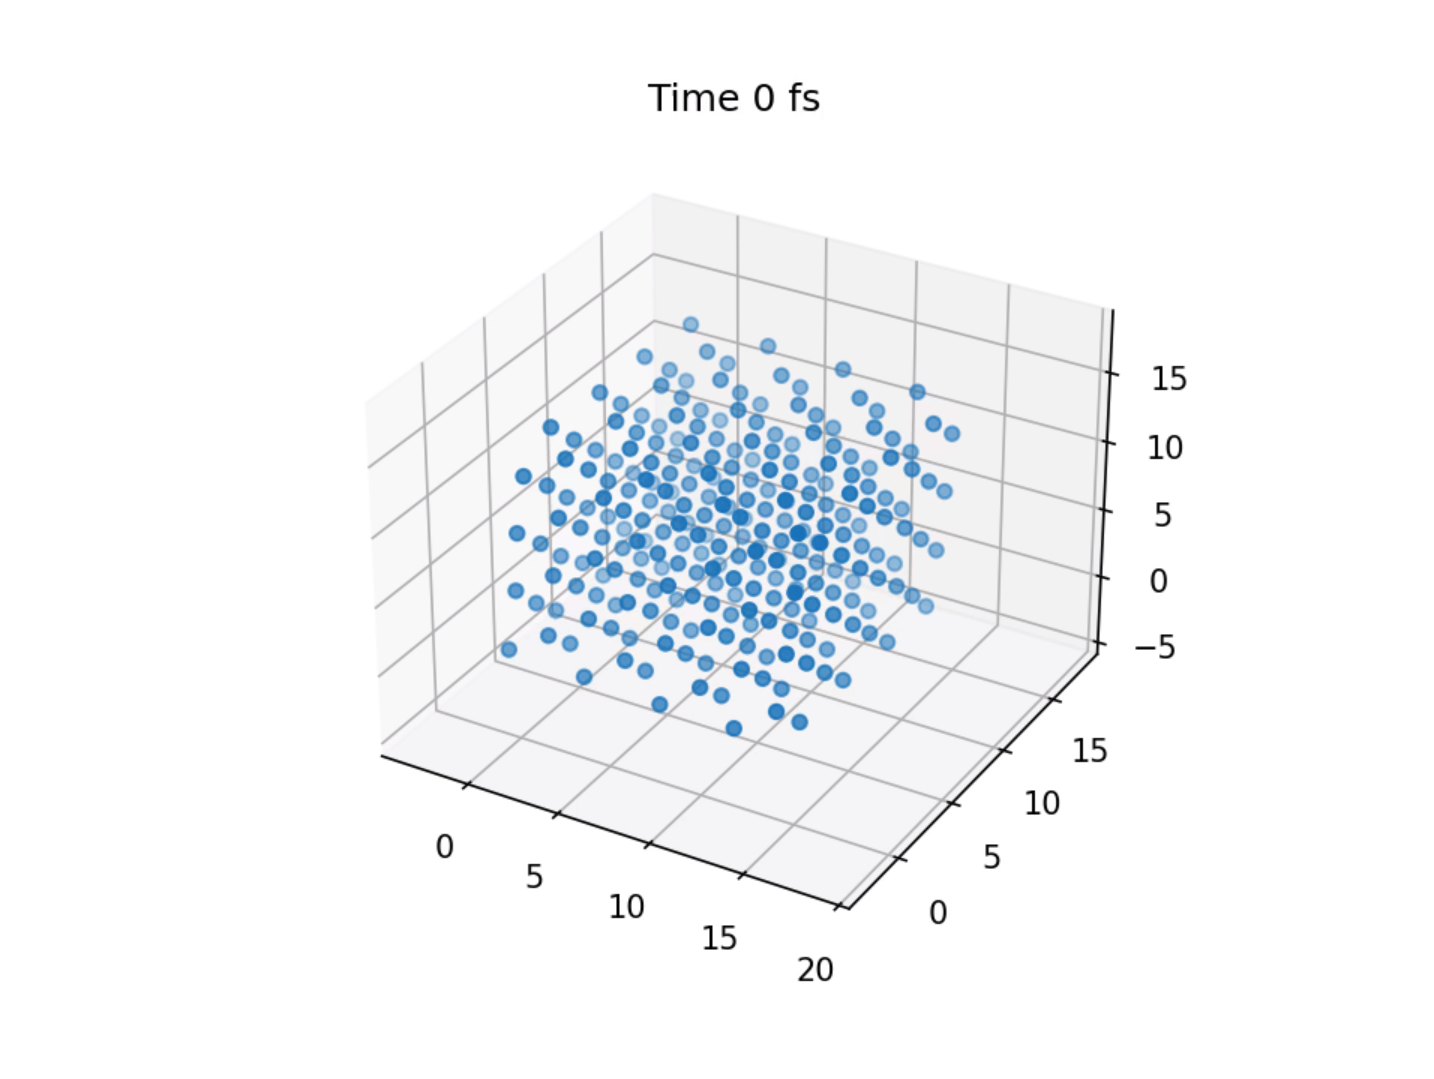
\includegraphics[width=0.7\textwidth]{images/thumbnail.png}
    \end{figure}

\end{frame}

\begin{frame}
    \frametitle{PBC, initial temperature}

    $$T_{init}=20\,K \rightarrow \langle T \rangle =10.001    \,K $$

    \begin{figure}
        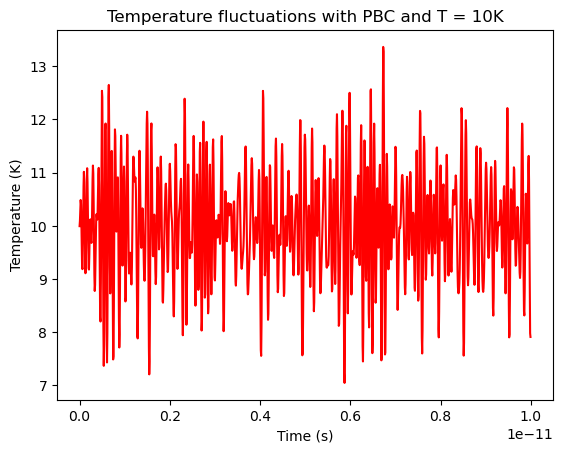
\includegraphics[width=0.7\textwidth]{images/temp5.png}
    \end{figure}

\end{frame}


\begin{frame}
    \frametitle{PBC, initial temperature}

    $$T_{init}=1550\,K \rightarrow \langle T \rangle =  800.6    \,K $$

    \begin{figure}
        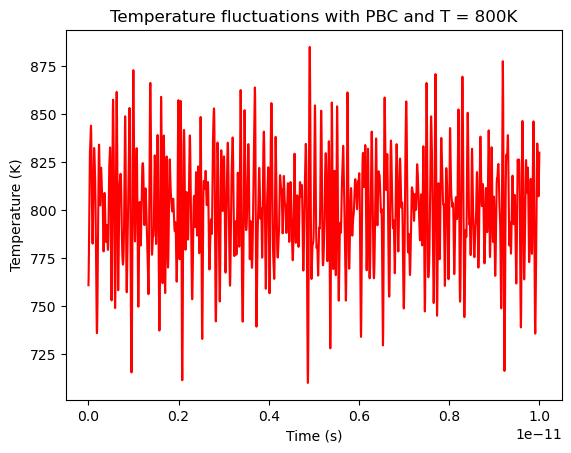
\includegraphics[width=0.7\textwidth]{images/temp5800k.png}
    \end{figure}

\end{frame}

\begin{frame}
    \frametitle{Extra atom trajectory, $T=1000\,K$}

    \begin{figure}
        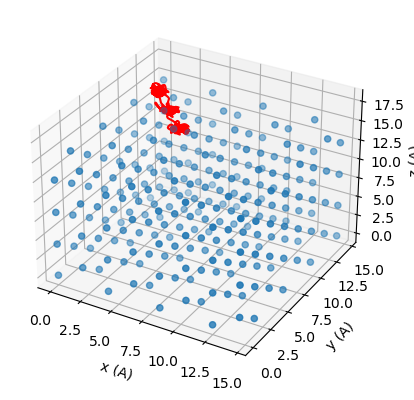
\includegraphics[width=0.7\textwidth]{images/extra1000k3d.png}
    \end{figure}

\end{frame}

\begin{frame}
    \frametitle{Extra atom trajectory, $T=1000\,K$}

    \centering Lateral view
    \begin{figure}
        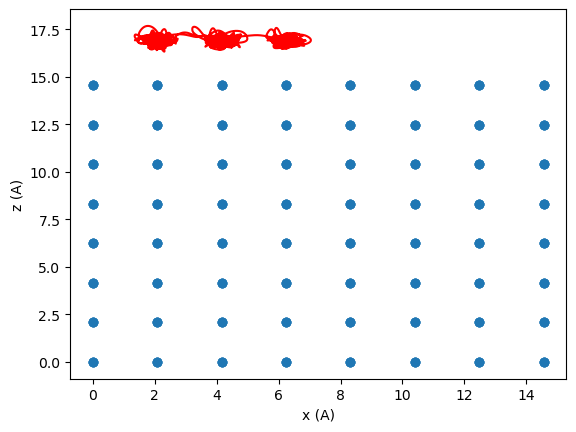
\includegraphics[width=0.7\textwidth]{images/extra1000klateral.png}
    \end{figure}

\end{frame}

\begin{frame}
    \frametitle{Extra atom trajectory, $T=1000\,K$}

    \centering View from above with only first layer
    \begin{figure}
        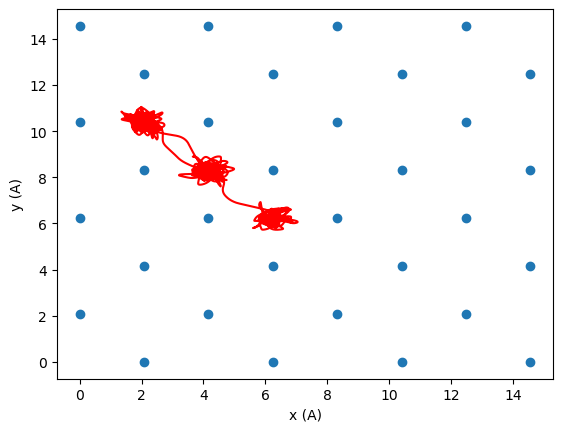
\includegraphics[width=0.7\textwidth]{images/extra1000kabove.png}
    \end{figure}

\end{frame}

\begin{frame}
    \frametitle{Extra atom trajectory, $T=600\,K$}

    \begin{figure}
        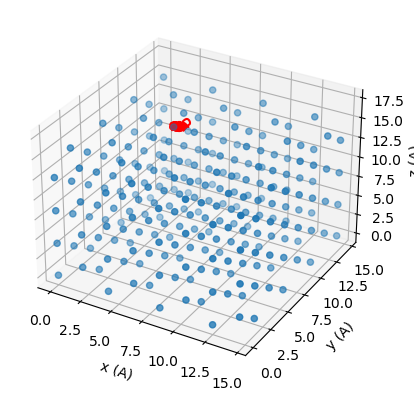
\includegraphics[width=0.7\textwidth]{images/extra600k3d.png}
    \end{figure}

\end{frame}

\begin{frame}
    \frametitle{Extra atom trajectory, $T=600\,K$}

    \centering Lateral view
    \begin{figure}
        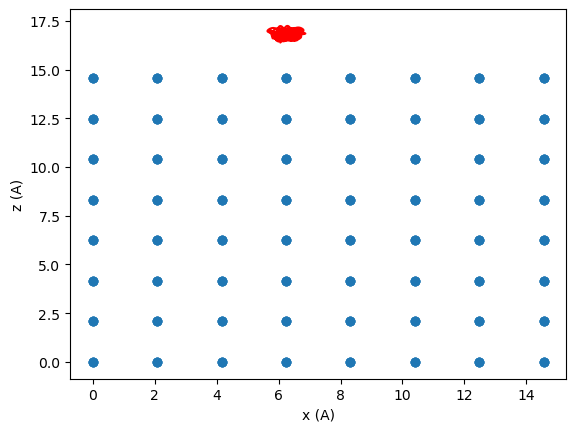
\includegraphics[width=0.7\textwidth]{images/extra600klateral.png}
    \end{figure}

\end{frame}

\begin{frame}
    \frametitle{Extra atom trajectory, $T=600\,K$}

    \centering View from above with only first layer
    \begin{figure}
        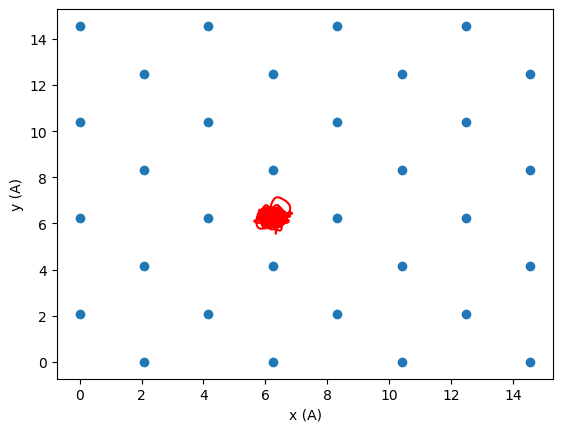
\includegraphics[width=0.7\textwidth]{images/extra600kabove.png}
    \end{figure}

\end{frame}

\end{document}